% !TeX spellcheck = cs_CZ
{\tikzset{external/prefix={tikz/FYZI/}}
 \tikzset{external/figure name/.add={ch14_}{}}
%---------------------------------------------------------------------------------------------------
% file fey1ch17.tex
%---------------------------------------------------------------------------------------------------
%=========================== Kapitola: Prostoročas ================================================
\chapter{Prostoročas}\label{fyz:IchapXVII}
\minitoc
  \section{Geometrie prostoročasu}\label{fyz:IchapXVIIsecI}
    Teorie relativity nám ukazuje, že vzájemné vztahy mezi naměřenými polohami a okamžiky ve dvou 
    různých souřadnicových soustavách nejsou takové, jaké bychom očekávali na základě našich 
    intuitivních představ. Je velmi důležité, abychom důkladně porozuměli vztahům mezi prostorem a 
    časem, jež vyplývají z Lorentzovy transformace, a proto se jim budeme v této kapitole věnovat 
    podrobněji.
    
    Lorentzova transformace mezi souřadnicemi a časem \newline\((x, y, z, t)\) naměřenými 
    pozorovatelem v „klidu“ a jim odpovídajícími souřadnicemi a časem \((x', y, z', t')\) 
    naměřenými uvnitř kosmické lodě, která se „pohybuje“ rychlostí \(u\) je
    \begin{equation}\label{FYZ:eq220}
      x' = \frac{x - ut}{\sqrt{1-\dfrac{u^2}{c^2}}}, \quad
      y' = y, \quad z' = z,                         \quad
      t' = \frac{t-\dfrac{u}{c^2}x}{\sqrt{1-\dfrac{u^2}{c^2}}}. 
    \end{equation} 
    Porovnejme tyto rovnice s rovnicemi (\ref{FYZ:eq149}), které rovněž spojují měření ve dvou 
    soustavách, přičemž jedna z nich je \emph{pootočena} vzhledem k druhé:
    \begin{equation}\label{FYZ:eq221}
      x' = x\cos\vartheta + y\cos\vartheta, \quad
      y' = y\cos\vartheta - x\sin\vartheta, \quad
      z' = z.
    \end{equation}
    V tomto konkrétním případě jsou souřadnicová osa \(x'\), kterou používá Pavel a souřadnicová 
    osa \(x\), kterou používá Petr pootočeny o úhel \(\vartheta\). Všimněme si, že v obou případech 
    jsou čárkované veličiny kombinací nečárkovaných: nové \(x'\) je kombinací \(x\) a \(y\) a nové 
    \(y'\) je kombinací \(x\) a \(y\).
    
    Zde je užitečná tato analogie: Díváme-li se na předmět, přirozeně u něho rozlišujeme to, co 
    můžeme nazvat „zdánlivá šířka“ i hloubka. Tyto dvě charakteristiky, šířka a hloubka, nejsou  
    \emph{základními} vlastnostmi předmětu, neboť když od něj odstoupíme a podíváme se na něj z 
    jiného úhlu, vidíme jinou šířku a jinou hloubku a mohli bychom si odvodit vzorce pro výpočet 
    nových charakteristik pomocí starých a pomocí úhlu pootočení. Těmito vzorci jsou rovnice 
    (\ref{FYZ:eq221}). Mohli bychom říci, že daná hloubka je určitou kombinací všech hloubek a 
    všech šířek. Kdybychom se vůbec nemohli pohybovat, daný předmět bychom vždy viděli ze stejného 
    místa a takové kombinování šířky a hloubky by nemělo smysl, neboť vždy bychom viděli tu 
    „pravou“ šířku a „pravou“ hloubku a zdálo by se nám, že to jsou zcela různé veličiny, neboť 
    jedna souvisí s úhlem, pod kterým vidíme předmět a druhá vyžaduje zaostření očí nebo dokonce 
    intuici. Zdálo by se, že jsou to dvě velmi odlišné věci a nikdy by se vzájemně nemíchaly. Jen 
    proto, že můžeme předmět obejít, si uvědomujeme, že hloubka a šířka jsou vlastně dvě různé 
    stránky téže věci.
     
    \emph{Nemůžeme se podobně podívat na Lorentzovu transformaci?} I tady se vyskytuje kombinace - 
    polohy a času. Z rozdílu mezi prostorovým a časovým měřením můžeme určit novou souřadnici 
    polohy. Jinak řečeno, v měřeních prostoru provedených jedním pozorovatelem je z hlediska jiného 
    pozorovatele malá složka času. Naše analogie nám dovoluje vyslovit tuto myšlenku: „realita“ 
    předmětu, na který se díváme, je o něco více (řečeno nepřesně a intuitivně) než jeho „šířka“ a 
    „hloubka“, neboť ty \emph{závisí} na tom, jak se na předmět díváme. Když přejdeme na nové 
    místo, náš mozek ihned přepočítává hloubku a šířku. Ale když se budeme pohybovat velkou 
    rychlostí, náš mozek nebude ihned přepočítávat souřadnice a čas. Nemáme praktickou zkušenost z 
    pohybu rychlostmi blízkými rychlosti světla, abychom si uvědomili fakt, že čas a prostor mají 
    stejnou podstatu. Je to něco podobného, jako kdybychom byli připoutáni na takové místo, ze 
    kterého bychom viděli jen šířku něčeho a nebyli schopni pootočit hlavu na jednu nebo druhou 
    stranu. Nyní chápeme, že kdybychom měli takovou možnost, mohli bychom vidět něco z času druhého 
    člověka - viděli bychom takříkajíc trošku „dozadu“.

    \begin{figure}[ht!]  %\ref{fyz:fig126}
      \centering
      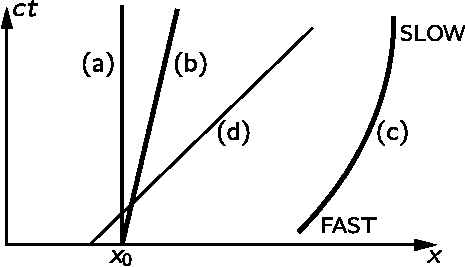
\includegraphics[width=0.7\linewidth]{fyz_fig126.pdf}
      \caption{Tři trajektorie částice v prostoročase: a) částice v klidu v bodě \(x = x_0\)
               b) částice, která vychází z bodu \(x = x_0\) a pohybuje se konstantní rychlostí
               c) částice, která letí zpočátku rychle a pak se přibrzdí d) trajektorie světla 
               \cite[s.~238]{Feynman01}}
      \label{fyz:fig126}
    \end{figure}
    
    Pokusme se tedy představit si předměty v novém světě. Prostor a čas jsou v něm vzájemně 
    kombinovány ve stejném smyslu, jak se na reálné předměty našeho obyčejného prostorového světa 
    můžeme dívat z různých směrů. Budeme si představovat, že předměty, nacházející se v prostoru, 
    které existují po určitou dobu, tvoří v novém světě jakési „hrudky“, a když se pohybujeme 
    různou rychlostí, vidíme takovou „hrudku“ z různých hledisek. Tento nový svět, tuto 
    geometrickou entitu, v níž existují „hrudky“ nacházející se na nějakém místě v určitém čase, 
    nazýváme \textbf{prostoročasem} (\emph{space-time}). Daný bod \((x, y, z, t)\) v prostoročase 
    se nazývá \textbf{událostí} (\emph{event}). Představme si například, že osu \(x\) znázorníme 
    graficky horizontálně, osy \(y\) a \(z\) ve dvou dalších směrech navzájem kolmých a kolmých i k 
    rovině papíru (!), a časovou osu vertikálně. Jak se na takovém grafu znázorní pohyb částice? 
    Jestliže se částice nepohybuje, má určitou souřadnici \(x\), a jak plyne čas, \(x\) se nemění, 
    takže její „trajektorie“ je čára rovnoběžná s osou \(t\) (obr. \ref{fyz:fig126}a). Na druhé 
    straně, jestliže se částice vzdaluje, pak \(x\) s rostoucím časem roste (obr. 
    \ref{fyz:fig126}b). Takže například pohyb částice, která se začne vzdalovat a pak se zpomaluje, 
    by se znázornil podobně jako na obr. \ref{fyz:fig126}c. To znamená, že částice, která je 
    stabilní a nerozpadá se, se v prostoročase zobrazí pomocí čáry. Částice, která se rozpadá, by 
    se zobrazila pomocí \emph{vidlice}, neboť se rozpadá na dvě další částice vycházející z jednoho 
    bodu.
    
    A co světlo? Světlo se šíří rychlostí \(c\), což se zobrazí přímkou s určitým konstantním 
    sklonem (obr. \ref{fyz:fig126}d).
    
    \begin{figure}[ht!]  %\ref{fyz:fig127}
      \centering
      \begin{tabular}{cc}
        \subfloat[nesprávně]{\label{fyz:fig127a}
          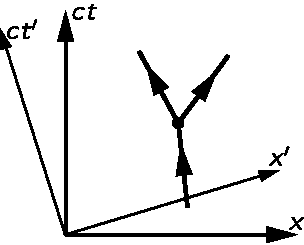
\includegraphics[width=0.4\linewidth]{fyz_fig127a.pdf}}
        \hspace{0.1\linewidth}                                                       &
        \subfloat[správně]{\label{fyz:fig127b}
          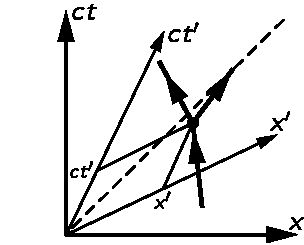
\includegraphics[width=0.4\linewidth]{fyz_fig127b.pdf}}
      \end{tabular}
      \caption{Dva pohledy na rozpadající se částici
               (\cite[s.~239]{Feynman01})}
      \label{fyz:fig127}
    \end{figure}
    
    Má-li tato představa vůbec smysl, očekávali bychom podle ní, že nastane-li s částicí nějaká 
    událost, například když se částice najednou rozpadne v daném bodě prostoročasu \((x, t)\) na 
    dvě nové částice letící po nových trajektoriích, stačí nám vzít novou dvojici souřadnicových 
    os, pootočit je a dostaneme nové \(t\) a nové \(x\) v novém systému, jak je to na obrázku 
    \ref{fyz:fig127a}. Ale to není pravda, neboť transformace (\ref{fyz:fig126}) není přesně 
    stejnou transformací jako (\ref{fyz:fig127}). Všimněme si například rozdílu v znameních a 
    skutečnosti, že jedna transformace obsahuje \(\cos\vartheta\) a \(\sin\vartheta\), zatímco 
    druhá obsahuje algebraické výrazy. (Samozřejmě není vyloučeno, že by se algebraické výrazy 
    nedaly vyjádřit pomocí funkce \(\cos\) a \(\sin\), ale v tomto případě to skutečně nejde.) 
    Přesto si však jsou obě transformace velmi podobné. Jak uvidíme, v důsledku rozdílnosti znamení 
    není geometrie v prostoročase obyčejnou reálnou geometrií. Opravdu, ačkoli jsme to 
    nezdůraznili, Ukazuje se, že pohybující se pozorovatel musí používat osy, které svírají stejný 
    úhel s prostoročasovou trajektorií světelného paprsku, přičemž své \(x'\) a \(t'\) určí pomocí 
    paralelní projekce do os \(x'\) a \(t'\), jak to je znázorněno na obr. \ref{fyz:fig127b}. Touto 
    geometrií se nebudeme zabývat, neboť by nám příliš nepomohla; snadněji se pracuje přímo s 
    rovnicemi.
    
  \section{Prostoročasové intervaly}\label{fyz:IchapXVIIsecII}
    Ačkoli geometrie prostoročasu není euklidovskou geometrií, přece je jí velmi podobná, až na 
    jisté zvláštnosti. Je-li tato koncepce geometrie správná, měly by existovat takové funkce 
    souřadnic a času, které nezávisí na souřadnicové soustavě. Například, vezmeme-li při obyčejných 
    rotacích dva body (pro jednoduchost nechť je jeden v počátku a druhý někde jinde) a obě 
    soustavy budou mít společný počátek, vzdálenost od počátku k druhému bodu bude v obou 
    soustavách stejná. Je to vlastnost, jež nezávisí na tom, ve které soustavě měříme. Druhá 
    mocnina vzdálenosti je \(x^2 + y^2 + z^2\). Jak je to s prostoročasem? Není těžké dokázat, že i 
    zde máme něco, co se nemění. Je to kombinace \(c^2t^2 - x^2 - y^2 - z^2\), která je stejná před 
    transformací i po ní:
    \begin{equation}\label{FYZ:eq222}
      c^2t'^2 - x'^2 - y'^2 - z'^2 = c^2t^2 - x^2 - y^2 - z^2.
    \end{equation}
    Tato veličina je proto něco, co podobné jako vzdálenost, je v jistém smyslu \uv{reálné}. Nazývá 
    se \textbf{intervalem} mezi dvěma prostoročasovými body, z nichž jeden je v tomto případě v 
    počátku. (Jde vlastně o druhou mocninu intervalu, podobně jako \(x^2 + y^2 + z^2\) je druhá 
    mocnina vzdálenosti.) Jiný název používáme proto, že jde o jinou geometrii, ale zajímavé je 
    jenom to, že některá znamení jsou opačná a je tam \(c\).
    
    Zbavme se \(d\). Chceme-li mít báječný prostor, kde \(x\) a \(y\) je možné vzájemně zaměnit, je 
    \(c\) absurdní. Vzniká tím zmatek, jako kdyby někdo nezkušený chtěl měřit šířku v zorných 
    úhlech a hloubku podle napětí při] zaostřování očních svalů a nakonec by vycházela třeba 
    hloubka ve stopách a šířka v metrech\footnote{Jednou z příčin neúspěchu americké sondy k Marsu 
    v r. \num{1999} bylo to, že část odborníků měřila ve stopách a část v metrech.}. Transformace, 
    jako je např. (\ref{FYZ:eq221}), vyjde pak nesmírně komplikovaně a celá jednoduchost a jasnost 
    se ztratí z prosté technické příčiny, že stejná věc se měřila ve dvou různých jednotkách. V 
    rovnicích (\ref{FYZ:eq220}) a (\ref{FYZ:eq222}) nám příroda říká, že \textbf{čas a prostor jsou 
    ekvivalentní} - čas se stává prostorem. \emph{Měly by se proto měřit ve stejných jednotkách}. 
    Jaká vzdálenost je „sekunda“? Ze (\ref{FYZ:eq222}) to lze snadno zjistit. Je to \num{3e8} 
    metrů, tj. \emph{vzdálenost, kterou urazí světlo za jednu sekundu}. Kdybychom všechny 
    vzdálenosti a časy měřili ve stejných jednotkách - sekundách, jednotkou vzdálenosti by pak bylo 
    \num{3e8} metrů a rovnice by byly jednodušší. Jiný způsob, jak sjednotit jednotky je měřit čas 
    v metrech. Co je to metr času? Metr časuje doba, kterou potřebuje světlo, aby uletělo 
    vzdálenost jeden metr, je tedy roven \SI{1/3e-8}{\s} nebo \num{3.3} miliardtiny sekundy! Jinými 
    slovy, rádi bychom naše rovnice napsali v takové soustavě jednotek, kde \(c = 1\). Měří-li se 
    čas a prostor v týchž jednotkách (jak to navrhujeme), pak je zřejmé, že rovnice se velmi 
    zjednodušší:
    \begin{equation}\label{FYZ:eq223}
      x' = \frac{x - ut}{\sqrt{1-u^2}},              \quad
      y' = y, \quad z' = z,                          \quad
      t' = \frac{t-ux}{\sqrt{1-u^2}} 
    \end{equation}
    \begin{equation}\label{FYZ:eq224}
      t'^2 - x'^2 - y'^2 - z'^2 = t^2 - x^2 - y^2 - z^2.
    \end{equation}
    Nemáme-li jistotu, nebo se obáváme, že tím, že zavedeme soustavu jednotek s \(c= 1\), už nikdy 
    nebudeme umět napsat naše rovnice správně, odpověď je zcela opačná. Rovnice se mnohem snadněji 
    zapamatují, když v nich nevystupuje \(c\), které lze vždy snadno dosadit zpět, podíváme-li se 
    na fyzikální rozměr. Tak například víme, že ve výrazu \(\sqrt{1 - u^2}\) nemůžeme odečítat 
    druhou mocninu rychlosti, která má svůj rozměr, od bezrozměrné jednotky. Proto \(u^2\) musíme 
    vydělit \(c^2\), abychom ho udělali bezrozměrným. Tak se to obecně dělá.
    
    Velmi zajímavý je rozdíl mezi prostoročasem a obyčejným prostorem, mezi intervalem a 
    vzdáleností. Podle vztahu (\ref{FYZ:eq224}), máme-li bod, jenž měl vdané souřadnicové soustavě 
    nulovou časovou souřadnici a má jen prostorové souřadnice, pak druhá mocnina intervalu bude 
    záporná a interval bude imaginární - druhá odmocnina ze záporného čísla. Intervaly mohou být 
    buď reálné, nebo imaginární. Na rozdíl od vzdálenosti, jejíž druhá mocnina je vždy kladná, může 
    být druhá mocnina intervalu kladná i záporná. Je-li interval imaginární, říkáme, že mezi dvěma 
    body je \textbf{prostoropodobný interval}, neboť se více podobá prostoru než času. Na druhé 
    straně, jsou-li dva body na stejném místě v dané souřadnicové soustavě a liší se jen časem, pak 
    druhá mocnina času je kladná, vzdálenosti jsou nulové a druhá mocnina intervalu je kladná - jde 
    o \textbf{časopodobný interval}. Náš prostoročasový diagram bude tedy vypadat takto: jsou na 
    něm dvě přímky pod úhlem \SI{45}{\degree} (jež jsou ve čtyřrozměrném prostoru vlastně kužely) a 
    všechny body na těchto přímkách mají nulový interval od počátku. Jak vidíme z rovnice 
    (\ref{FYZ:eq224}), místa, kterými prochází světlo vyslané z daného bodu, jsou od toho bodu 
    vzdálena o nulový interval. Shodou okolností jsme právě dokázali, že šíří-li se světlo 
    rychlostí \(c\) v jedné soustavě, šíří sejí i v druhé soustavě, neboť je-li interval v obou 
    soustavách stejný, tj. v obou nulový, pak výpověď, že rychlost šíření světla je invariantní, je 
    stejná, jako když řekneme, že interval je roven nule.
    
  \section{Minulost, přítomnost a budoucnost}\label{fyz:IchapXVIIsecIII}
    Prostoročas v okolí daného prostoročasového bodu lze rozdělit na tři oblasti znázorněné na obr. 
    \ref{fyz_fig128}. V jedné oblasti máme prostoropodobné intervaly a ve dvou oblastech 
    časopodobné intervaly. Co se týká fyziky, pak tyto tři oblasti, na něž je rozdělen prostoročas 
    v okolí daného bodu, k němu mají zajímavý fyzikální vztah. Fyzické těleso nebo signál se může 
    dostat z bodu v oblasti \(2\) do události \(O\), pohybuje-li se pomaleji než rychlostí světla.

    \begin{figure}[ht!] %\ref{fyz_fig128}
      \centering
      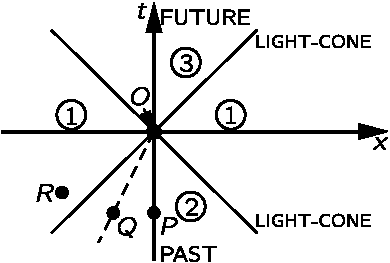
\includegraphics[width=0.7\linewidth]{fyz_fig128.pdf}
      \caption{Část prostoročasu v okolí počátku
               (\cite[s.~241]{Feynman01})}
      \label{fyz_fig128}
    \end{figure}
    
    Proto události v této oblasti mohou ovlivnit bod \(O\), mohou ho ovlivnit z minulosti. Událost 
    v bodě \(P\) na záporné ose \(t\) je přesně v „minulosti“ vzhledem k \(O\). Je to stejný 
    prostorový bod, jen o něco dříve. Co se tam událo tehdy, ovlivňuje \(O\) nyní. (Bohužel, takový 
    je už život). Jiný předmět v bodě \(Q\) se může dostat do \(O\), pohybuje-li se určitou 
    rychlostí menší než \(c\). Jestliže tento předmět byl v kosmické lodi a pohyboval se, může 
    představovat minulost bodu \(O\), tj. v jiné souřadnicové soustavě může jít časová osa body 
    \(O\) a \(Q\). Všechny body v oblasti \(2\) jsou v „minulosti“ vzhledem k \(O\) a cokoli se 
    stane v této oblasti, \emph{může} bod \(O\) ovlivnit. Proto se někdy oblast \(2\) nazývá 
    \emph{oblastí ovlivňující minulost}. Je to oblast událostí, jež mohou nějak ovlivnit bod \(O\).
    
    Na druhé straně, oblast \(3\) je taková, že ji můžeme ovlivnit z bodu \(O\). Vystřelením kulek 
    rychlostí menší než \(c\), můžeme zasáhnout předměty nacházející se v ní. Takže je to část 
    světa, jehož budoucnost můžeme ovlivnit, a proto ji můžeme nazvat \emph{oblastí ovlivnitelné 
    budoucnosti}. Co zajímavého můžeme říci o zbývající částí prostoročasu, tj. oblasti \(1\)? To, 
    že ji nemůžeme ovlivnit z bodu \(O\), ani ona nemůže ovlivnit nás v bodě \(O\), neboť nic se 
    nemůže pohybovat rychleji než světlo. Samozřejmě, co se stane v \(R\), \emph{může} nás ovlivnit 
    později. Kdyby Slunce explodovalo „právě teď“, trvalo by to osm minut, než bychom se to 
    dozvěděli, a v žádném případě by nás to nemohlo ovlivnit dříve.
    
    Co myslíme pojmem „právě teď“, je záhadná věc, kterou nemůžeme definovat ani ovlivnit. Ale 
    později může ovlivnit nás, nebo bychom ji byli mohli ovlivnit, kdybychom byli provedli něco 
    dostatečně dávno v minulosti. Když se díváme na hvězdu Alfa Centauri, vidíme, jak vypadala před 
    čtyřmi roky, a můžeme se jen dohadovat, jak vypadá „teď“. „Teď“ - znamená ve stejném okamžiku 
    v naší speciální souřadnicové soustavě. Alfa Centauri můžeme vidět jenom ve světle, jež k nám 
    přichází z minulosti před čtyřmi lety, ale nevíme, co se tam děje „teď“. Trvá to čtyři roky, 
    než to, co se tam děje teď, nás ovlivní. Alfa Centauri „teď“ je čistě námi vymyšlená idea, 
    pojem. Není to něco, co by se dalo momentálně fyzikálně definovat, neboť abychom to mohli 
    pozorovat, musíme počkat. Navíc „teď“ závisí na souřadnicové soustavě. Kdyby se například Alfa 
    Centauri pohybovala, pozorovatel, který by byl na ní, by s námi nesouhlasil, neboť jeho 
    souřadnice by s našimi svíraly nějaký úhel a jeho „teď“ by byl \emph{jiný} okamžik. O tom, že 
    současnost není nic jednoznačného, jsme již hovořili.
    
  \section{Podrobnosti o čtyřvektorech}\label{fyz:IchapXVIIsecIV}
    Vraťme se k naší úvaze o analogii mezi Lorentzovou transformací a rotacemi prostorových os. Při 
    konstrukci vektorů, směrovaných úseček, jsme poznali užitečnost hledání veličin, jež mají 
    stejné transformační vlastnosti jako souřadnice. V případě obyčejných rotací existuje mnoho 
    veličin, jež se transformují jako \(x\), \(y\), a \(z\). Například rychlost má tři složky 
    \(x\), \(y\) a \(z\); když ji popisujeme v nové souřadnicové soustavě, ani jedna ze složek není 
    stejná, ale všechny se přetransformují na nové hodnoty. Ale tak, či onak, sama rychlost je 
    jaksi reálnější než její jednotlivé složky a znázorňujeme ji směrovanou úsečkou.
    
    Proto se ptáme: Existují také veličiny, které se v pohybující se a klidové soustavě 
    transformují stejně jako \(x\), \(y\), \(z\) a \(t\)? Na základě naší zkušenosti s vektory 
    víme, že tři z těchto veličin, podobně jako \(x\), \(y\), \(z\), budou tvořit složky obyčejného 
    prostorového vektoru. Čtvrtá veličina se však bude při prostorových rotacích jevit jako 
    obyčejný skalár, protože se nemění, dokud nepřejdeme k pohybující se soustavě. Lze tedy k našim 
    známým „trojvektorům“ přiřadit čtvrtou veličinu (nazvali bychom ji „časovou složkou“) takovým 
    způsobem, že by čtyři veličiny „rotovaly“ tak jako poloha a čas v prostoročase? Nyní si ukažme, 
    že skutečně aspoň jedna takováto čtveřice existuje (ve skutečnosti jich je mnoho): \emph{tři 
    složky hybnosti a energie jako časová složka se spolu transformují} tak, že vytvářejí to, čemu 
    říkáme „čtyřvektor“. Protože je dost nepohodlné všude psát \(c\), použijeme na jednotky 
    energie, hmotnosti a hybnosti stejný trik, jaký jsme použili v rovnici (\ref{FYZ:eq223}). 
    Energie a hmotnost se například liší jen faktorem \(c^2\), což je pouze otázka jednotek, takže 
    můžeme říci, že energie je hmotnost. Místo toho, abychom psali \(c^2\), položíme \(E = m\), a 
    pak, kdyby byly nějaké potíže, můžeme do výsledné rovnice dodat potřebné množství \(c\), 
    abychom získali správné jednotky, ale v průběžných výpočtech je vynecháme. Tak dostaneme 
    rovnice pro energii a hybnost:
    \begin{equation}\label{FYZ:eq225}
      E = m = \dfrac{m_0}{\sqrt{1 - v^2}}, \qquad
      \vec{p} = m\vec{v} = \dfrac{m_0\vec{v}}{\sqrt{1 - v^2}}
    \end{equation}
    V těchto jednotkách máme i
    \begin{equation}\label{FYZ:eq226}
      E^2 - p^2 = m_0^2.
    \end{equation}
    
    Například, když měříme energii v elektronvoltech, jaká bude hmotnost jednoho elektronvoltu? Je 
    to hmotnost, jejíž klidová energie je \num{1} elektronvolt, tj. \(m_0c^2\) je jeden 
    elektronvolt. Například klidová hmotnost elektronu je \SI{0.511e6}{\electronvolt}.
    
    Jak bude vypadat energie a hybnost v nové souřadnicové soustavě? Abychom to zjistili, musíme 
    provést transformaci rovnice (\ref{FYZ:eq225}), což je možné, neboť víme, jak se transformuje 
    rychlost. Předpokládejme, že těleso má rychlost \(v\), ale my se na něj díváme z kosmické lodě, 
    jež se sama pohybuje rychlostí \(u\) a v této soustavě označujeme veličiny jako čárkované. 
    Abychom věc zjednodušili, uvažujme případ, kdy rychlost \(v\) má směr \(u\) (později můžeme 
    řešit obecnější případ). Jaké je \(v'\), tj. rychlost z hlediska kosmické lodě? Je to složená 
    rychlost, „rozdíl“ mezi \(v\) a \(u\). Podle zákona, který jsme odvodili dříve,
    \begin{equation}\label{FYZ:eq227}
      v' = \frac{v-u}{1-uv}.
    \end{equation}
    Dále vypočtěme novou energii \(E'\), tj. energii, jak ji určí pozorovatel v kosmické lodi! 
    Použije stejnou klidovou hmotnost, což je samozřejmé, ale pro rychlost použije \(v'\). 
    Potřebujeme umocnit \(v'\) na druhou, odečíst ji od jedné, odmocnit a vzít převrácenou hodnotu
    \begin{equation*}
      {v'}^2 = \frac{v^2 - 2uv + v^2}{1 - 2uv + u^2v^2},
    \end{equation*}
    \begin{align*}
      1 - {v'}^2 &= \frac{1 - 2uv + u^2v^2 - v^2 + 2uv - v^2}{1 - 2uv + u^2v^2}  \\
                 &= \frac{1 - v^2 - u^2 + u^2v^2}{1 - 2uv + u^2v^2}              \\
                 &= \frac{(1-u^2)(1-v^2)}{(1 - uv)^2}.
    \end{align*}
    Tedy
    \begin{equation}\label{FYZ:eq228}
      \frac{1}{\sqrt{1 - {v'}^2}} = \frac{1-uv}{\sqrt{1-u^2}\sqrt{1-v^2}}
    \end{equation}
    
    \begin{figure}[ht!] %\ref{fyz_fig129}
      \centering
      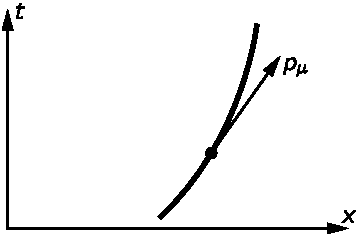
\includegraphics[width=0.5\linewidth]{fyz_fig129.pdf}
      \caption{Čtyřvektor hybnosti částice
               (\cite[s.~244]{Feynman01})}
      \label{fyz_fig129}
    \end{figure}
    
  \section{Čtyřvektorová algebra}\label{fyz:IchapXVIIsecV}
  \section{Příklady a cvičení}\label{fyz:IchapXVIIsecVI}

} %tikzset
%---------------------------------------------------------------------------------------------------
\printbibliography[title={Seznam literatury}, heading=subbibliography]
\addcontentsline{toc}{section}{Seznam literatury}